\newpage
\section{Configuring Certificate Auto-Enrollment}
\subsection{Activities}

\noindent {\bf{Bước 1:}} Khởi động máy ảo Windows được sử dụng trong phần 2.

\noindent {\bf{Bước 2:}} Mở PKI, thên snap-in \textbf{Group Policy Management} theo cách được sử dụng trong phần 2.

\begin{figure}[!htb]
    \centering
    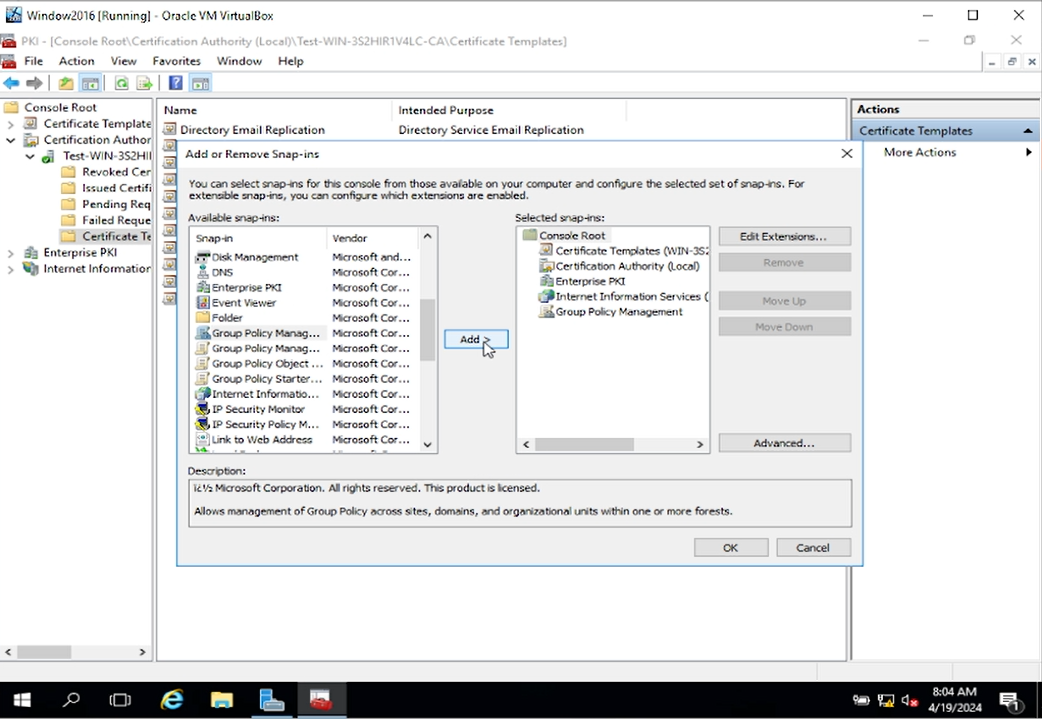
\includegraphics[width=0.7\linewidth]{figure//chapter4//lab4_3/add_group_policy_management.png}
    \caption{Thêm Group Policy Management}
    \label{fig:enter-label}
\end{figure}

\noindent {\bf{Bước 3:}} Ở PKI, mở rộng\textbf{Group Policy Management} > \textbf{Forest.local} > \textbf{Domains} > \textbf{Test.local}. Chuột phải \textbf{Default Domain Policy}, chọn \textbf{Edit}. 

\begin{figure}[!htb]
    \centering
    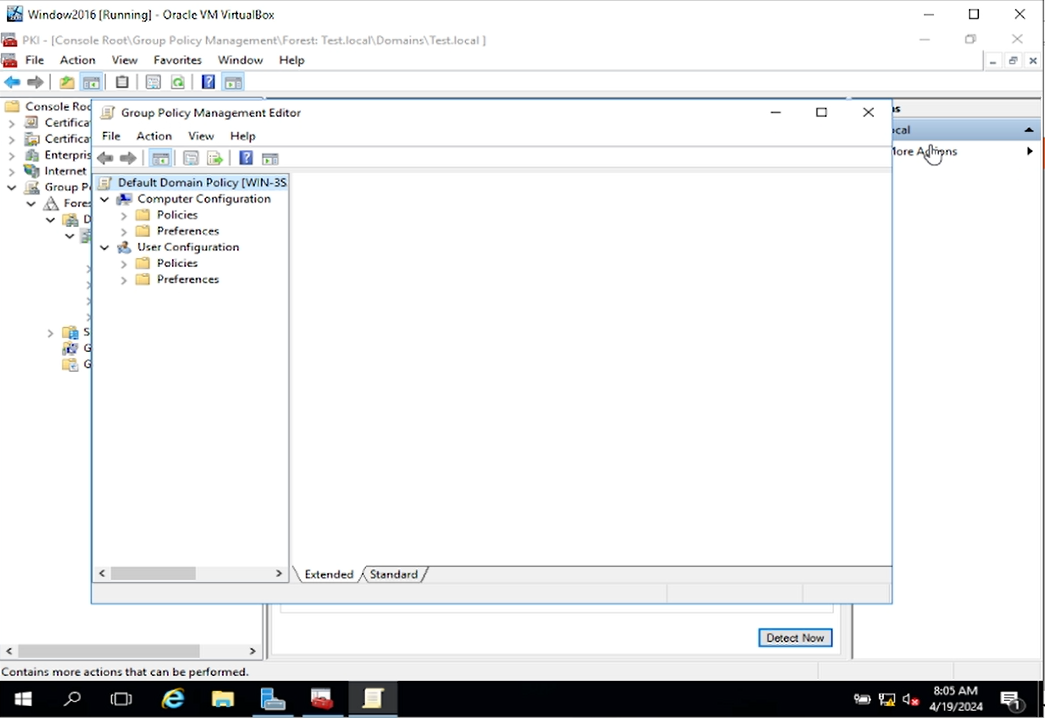
\includegraphics[width=0.8\linewidth]{figure//chapter4//lab4_3/gpm_editor.png}
    \caption{Màn hình Group Policy Management Editor}
    \label{fig:enter-label}
\end{figure}

Tiếp tục mở rộng theo thứ tự \textbf{User Configuration } > \textbf{Policies} > \textbf{Windows Settings} > \textbf{Security Settings} và chọn \textbf{Public Key Policies}.

\begin{figure}[!htb]
    \centering
    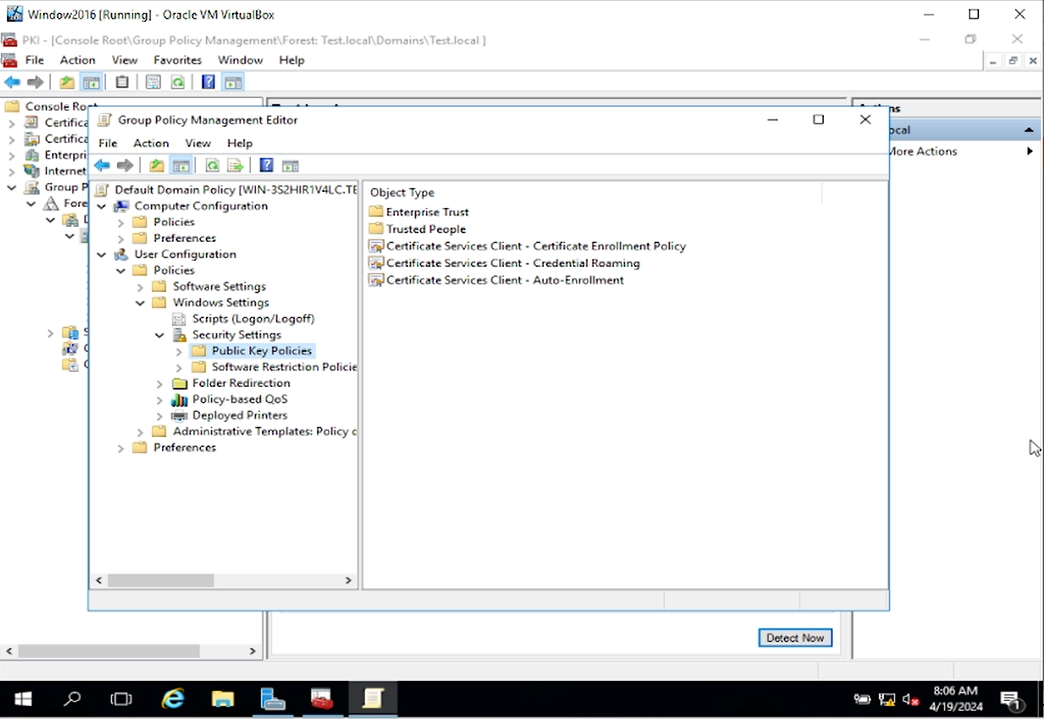
\includegraphics[width=0.8\linewidth]{figure//chapter4//lab4_3/public_key_policies.png}
    \caption{Public Key Policies}
    \label{fig:enter-label}
\end{figure}

Ở thanh bên phải, chuột phải vào \textbf{Certificate Services Client -  AutoEnrollment} và chọn \textbf{Properties}. Đặt \textbf{Configuration Model} thành \textbf{Enable} và chọn \textbf{Renew expired certificates, update pending certificates, and remove revoked certificates} và \textbf{Update certificates that use certificate templates}.

\begin{figure}[!htb]
    \centering
    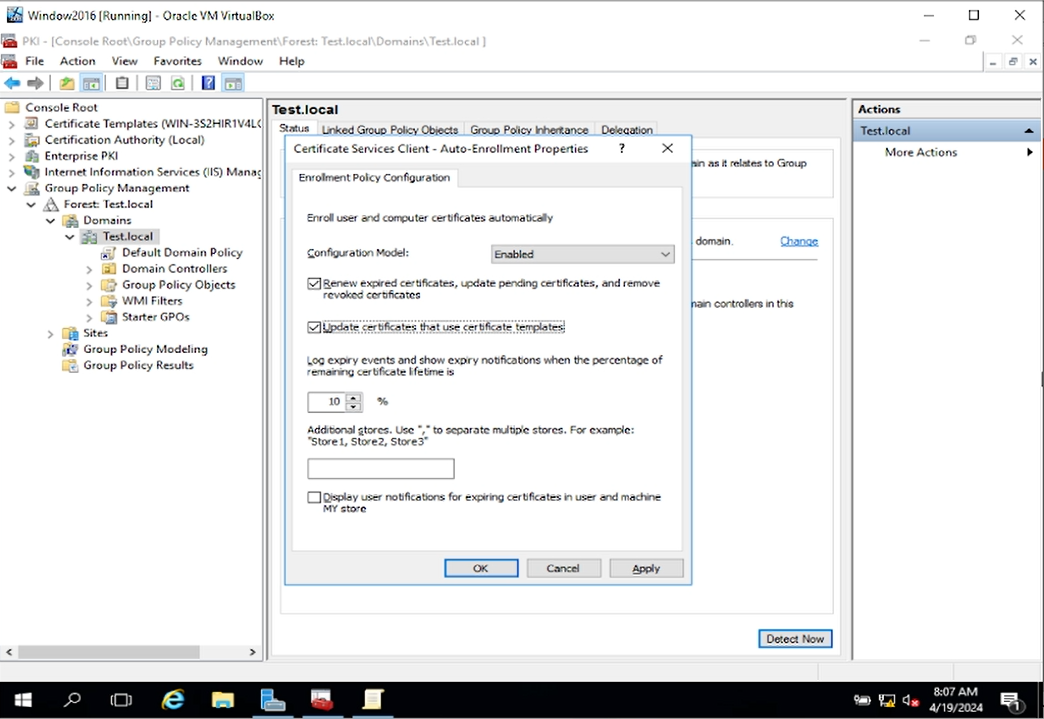
\includegraphics[width=0.8\linewidth]{figure//chapter4//lab4_3/cert_service_client_autoenrollment.png}
    \caption{Cấu hình Certificate Service Client Auto-Enrollment}
    \label{fig:enter-label}
\end{figure}

\newpage

\noindent {\bf{Bước 4:}} Ở PKI, mở rộng \textbf{Certification Authority (Local)} > ServerName, chọn \textbf{Certificate Templates}.

\begin{figure}[!htb]
    \centering
    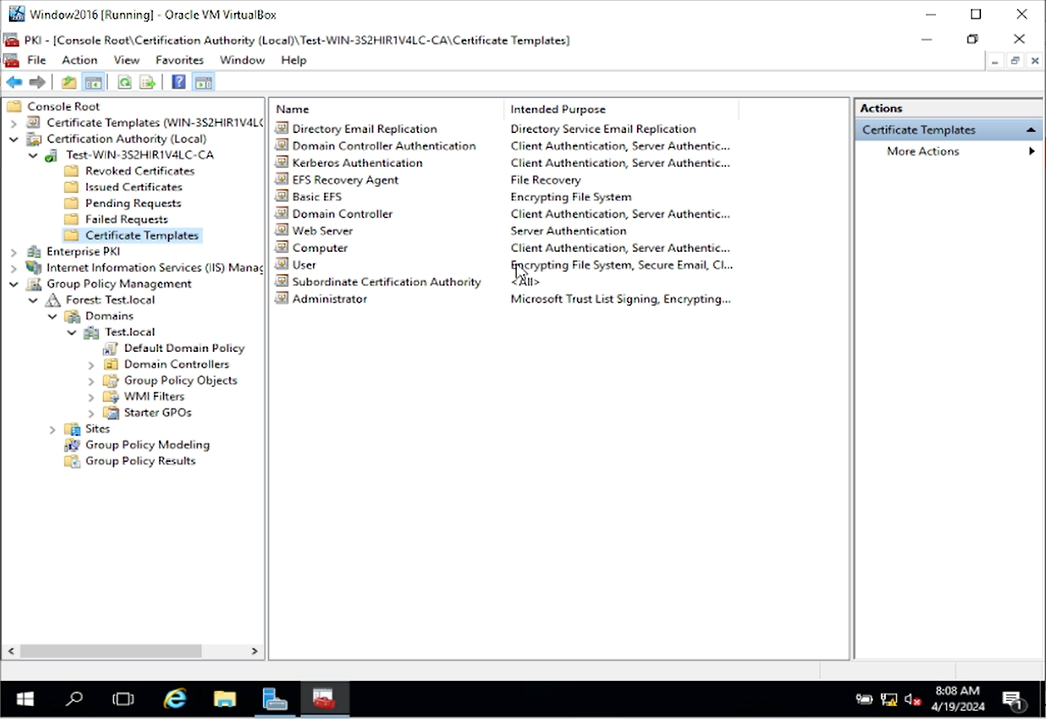
\includegraphics[width=0.9\linewidth]{figure//chapter4//lab4_3/cert_temp_in_auth.png}
    \caption{Màn hình Certificate Templates trong phần Certification Authority (Local)}
    \label{fig:enter-label}
\end{figure}

\noindent {\bf{Bước 5:}} Chọn \textbf{Certificate Templates} ở bên ngoài, chuột phải vào User và chọn \textbf{Duplicate Template}.

\begin{figure}[!htb]
    \centering
    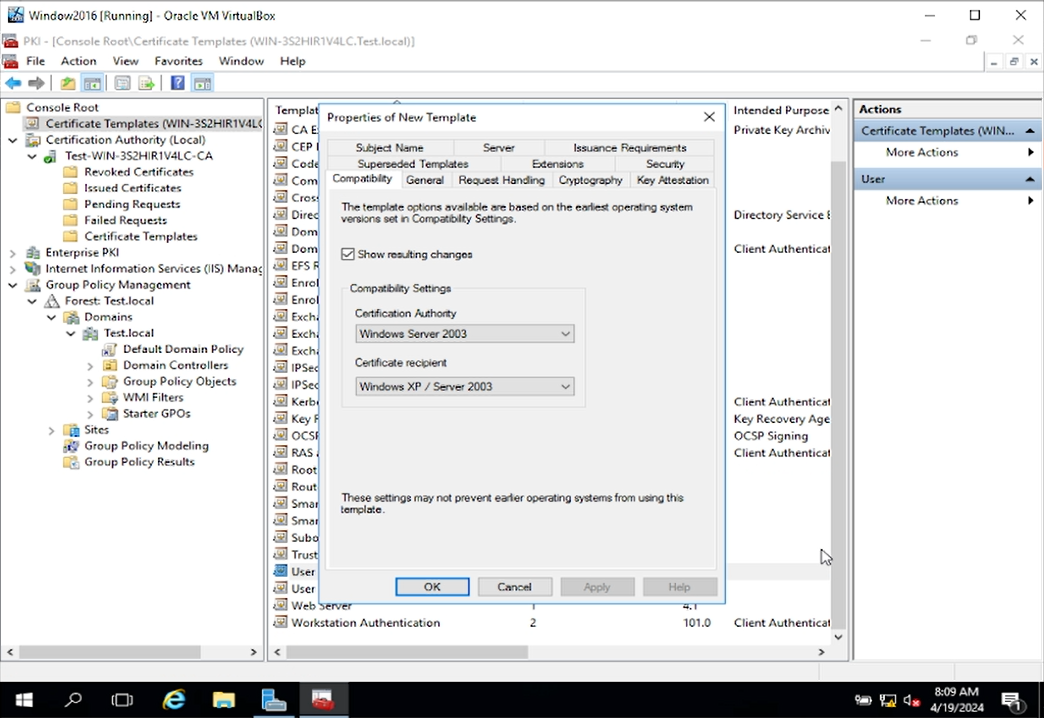
\includegraphics[width=0.9\linewidth]{figure//chapter4//lab4_3/duplicate_template.png}
    \caption{Màn hình Duplicate Template}
    \label{fig:enter-label}
\end{figure}

Ở \textbf{General}, chuyển \textbf{Template display name} thành \textbf{ServerName}, \textbf{Validity period number} thành 2 năm, và \textbf{Renewal period number} thành 12 tháng.

\begin{figure}[!htb]
    \centering
    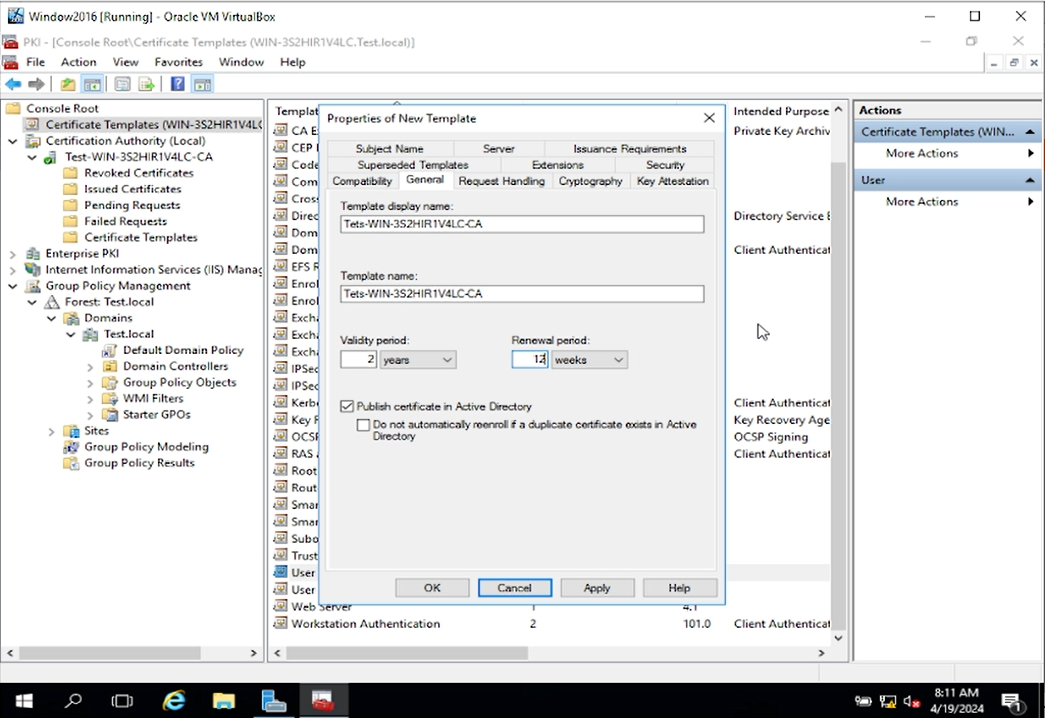
\includegraphics[width=0.9\linewidth]{figure//chapter4//lab4_3/general_tab.png}
    \caption{General Tab}
    \label{fig:enter-label}
\end{figure}

Ở \textbf{Request Handling}, chọn \textbf{Prompt the user during enrollment}.

\begin{figure}[!htb]
    \centering
    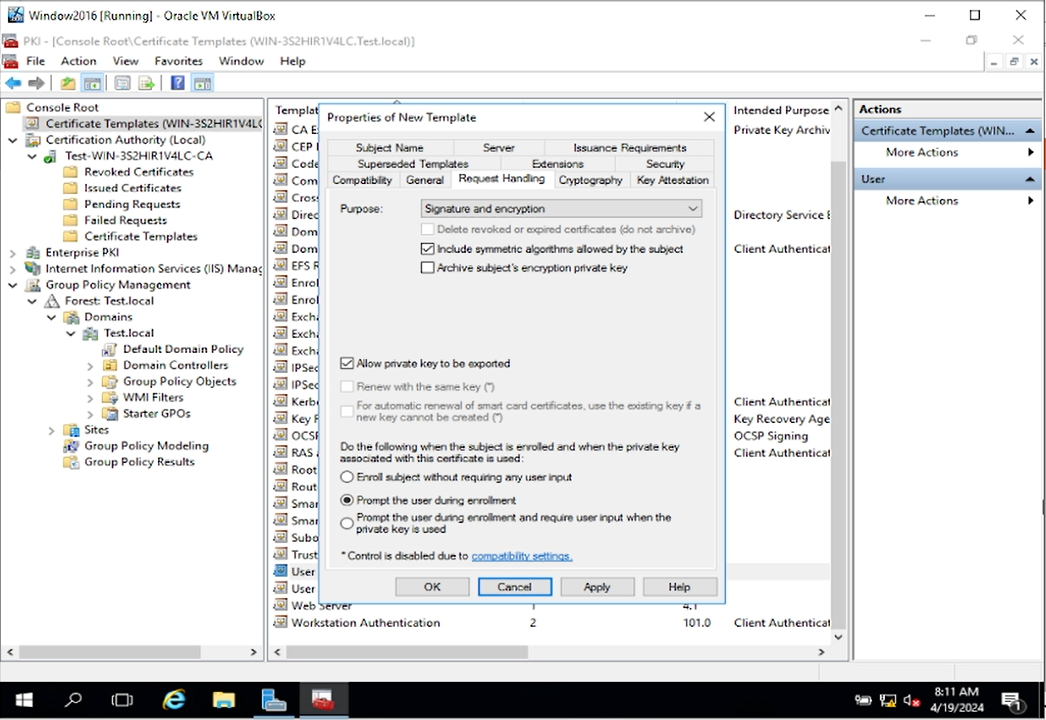
\includegraphics[width=0.9\linewidth]{figure//chapter4//lab4_3/request_handling.png}
    \caption{Request Handling Tab}
    \label{fig:enter-label}
\end{figure}

\noindent {\bf{Bước 6:}} Ở \textbf{Security}, chọn \textbf{Add}. Chuyển \textbf{Enter the object names to select box} thành \textbf{Anthony Newman} (Tài khoản đã được lập trước đó). Ở \textbf{Group or user names}, chọn Anthony Newman. Và ở \textbf{Permissions for Anthony Newman}, chọn \textbf{Allow} cho \textbf{Enroll} và \textbf{Autoenroll}.

\begin{figure}[!htb]
    \centering
    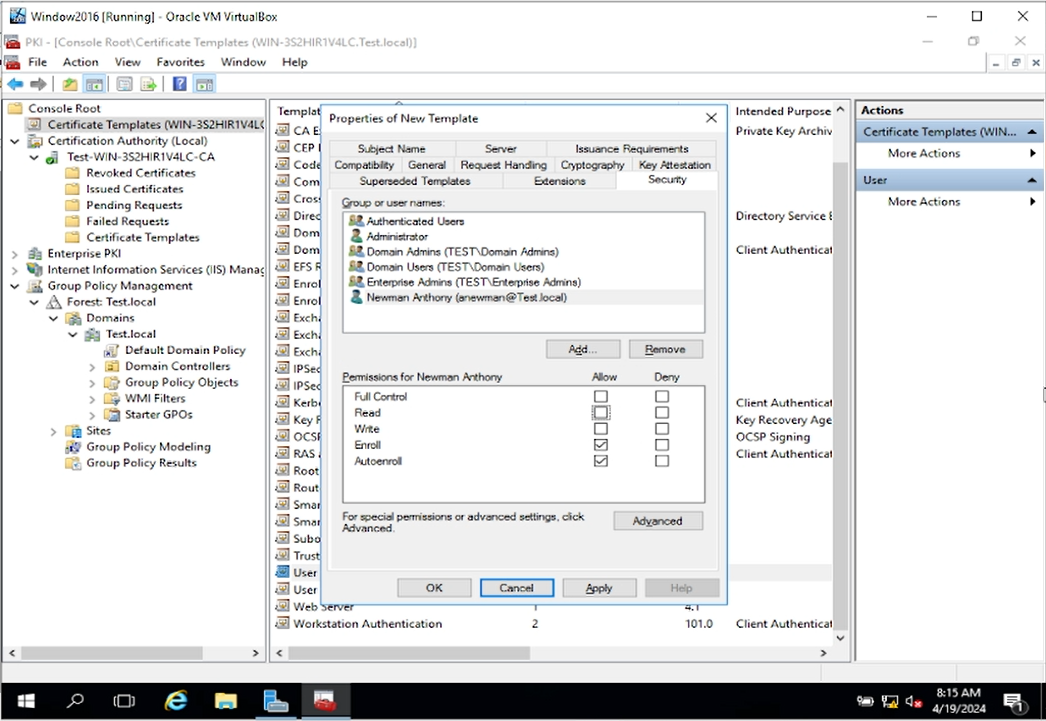
\includegraphics[width=0.7\linewidth]{figure//chapter4//lab4_3/security_tab.png}
    \caption{Security Tab}
    \label{fig:enter-label}
\end{figure}

\noindent {\bf{Bước 7:}} Quay lại \textbf{Certificate Templates} ở trong \textbf{Certification Authority (Local)}. Nhấn chuột phải và chọn \textbf{New}, chọn \textbf{Certificate Template to Issue}. Ở \textbf{Enable Certificate Templates}, chọn \textbf{ServerName}. Certificate mới sẽ xuất hiện ở \textbf{Certificate Templates}.

\begin{figure}[!htb]
    \centering
    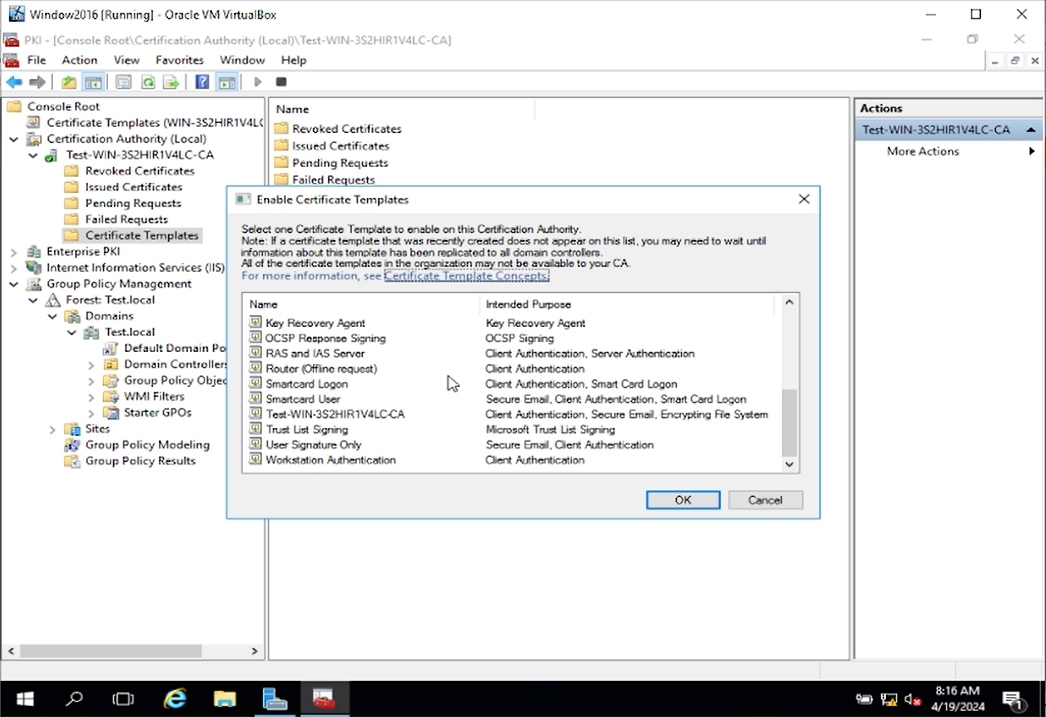
\includegraphics[width=0.7\linewidth]{figure//chapter4//lab4_3/enable_certificate.png}
    \caption{Màn hình Enable Certificate Templates}
    \label{fig:enter-label}
\end{figure}

Cuối cùng, có thể click vào \textbf{ServerName} để biết thêm chi tiết về Certificate này.

\subsection{Review Questions}

\noindent Câu 1: 

A: Users should export their public keys and store them in a safe place.

\noindent Câu 2: 

ii: Choose a certificate template that allow users to digitally sign emails.

B: you did not assign the global security group the View permission to the certificate template.

\noindent Câu 3: 

B: Once a User certificate is issued to a user, the best practice is to revoke the user's EFS certiciate.

\noindent Câu 4: True.

\noindent Câu 5:

B: Install Anthony's certificate.